\chapter{Modelling Networks with VDM in Multi-models}
\label{sec:networks}

In this section, we address the problem of modelling networked controllers in multi-models, presenting a solution using VDM. When modelling and designing distributed controllers, it is necessary to model communications between controllers as well. While controller FMUs can be connected directly to each other through for co-simulation, this quickly becomes unwieldy due to the number of connections increasing exponentially. For example, consider the case of five controllers depicted in Figure~\ref{fig:bigraph}. In order to connect each controller together, 20 connections are needed (i.e.\ for a complete bidirected graph). Even with automatic generation of multi-model configurations, this is in general not a feasible solution.

\begin{figure}[hb]
\centering
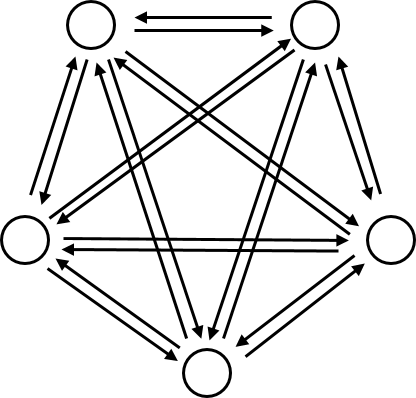
\includegraphics[scale=0.4]{figures/bigraph}
\caption{Topology of five controllers connected to each other}
\label{fig:bigraph}
\end{figure}

We suggest employing a pattern described initially as part of the Crescendo technology~\cite{Fitzgerald&14c}, in which a representation of an abstract communications medium called the `ether' is introduced. In the INTO-CPS setting, the ether is an FMU that is connected to each controller that handles message-passing between them. This reduces the number of connections needed, particularly for large numbers of controllers such as swarms. For five controllers, only 10 connections are needed, as shown in Figure~\ref{fig:bigraph2}.

\begin{figure}[hb]
\centering
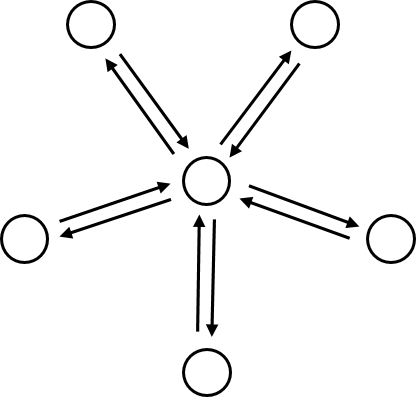
\includegraphics[scale=0.4]{figures/bigraph2}
\caption{Topology of five controllers connected via a shared medium}
\label{fig:bigraph2}
\end{figure}

In the remainder of this section, we describe how to pass messages between VDM FMUs using string types, how the ether class works, some of the consequences of using the ether pattern, and finally some extensions for providing quality of service (QoS) guarantees. %A class listing for a reference implementation of the \texttt{Ether} class is given in Appendix~\ref{app:ether}.
An example multi-model, called \emph{Case Study: Ether}, is available from the INTO-CPS Application. It is also described in the Examples Compendium, Deliverable D3.6~\cite{INTOCPSD3.6}.

\section{Representing VDM Values as Strings}

Connections between FMUs are typically numerical or Boolean types. This works well for modelling of discrete-time (DT) controllers and continuous-time (CT) physical models, however one of the advantages of VDM is the ability to represent more complex data types that better fit the abstractions of supervisory control. Therefore, in a multi-modelling setting, it is advantageous if VDM controllers can communicate with each other using data types that are not part of the FMI specification.

This can be achieved by passing strings between VDM FMUs (which are now supported by the Overture FMU export plug-in) and the \texttt{VDMUtil} standard library included in Overture, which can convert VDM types to their string representations and back again.

The \texttt{VDMUtil} library provides a (polymorphic) function called \texttt{val2seq\_of\_char}, that converts a VDM type to a string. It is necessary to tell the function what type to expect as a parameter in square brackets. For example, in the following listing, a 2-tuple is passed to the function, which will produce the output \texttt{"mk\_(2.4, 1.5)"}:

\begin{vdm}
VDMUtil`val2seq_of_char[real*real](mk_(2.4, 1.5))
\end{vdm}

The above can be used when sending messages as strings. In the model receiving message, the inverse function \texttt{seq\_of\_char2val} can be used. This function returns two values, a Boolean value indicating if the conversion was successful, and the value that was received:

\begin{vdm}
let mk_(b,v) = VDMUtil`val2seq_of_char[real*real](msg) in
  if b then ...
\end{vdm}

In the first few steps of co-simulation, empty or invalid strings are often passed as values, so it is necessary to check if the conversion was successful (as in the above listing) before using the value.

Note that currently (as of Overture 2.4.0), the \texttt{VDMUtil} library is called in the default scope, meaning that it does not know about custom types defined in the model. Therefore, it is recommended to pack values in a tuple (as in the above example) for message passing, then convert to and from any custom types in the sending and receiving models.

\section{Using the Ether FMU}

\begin{figure}
\centering
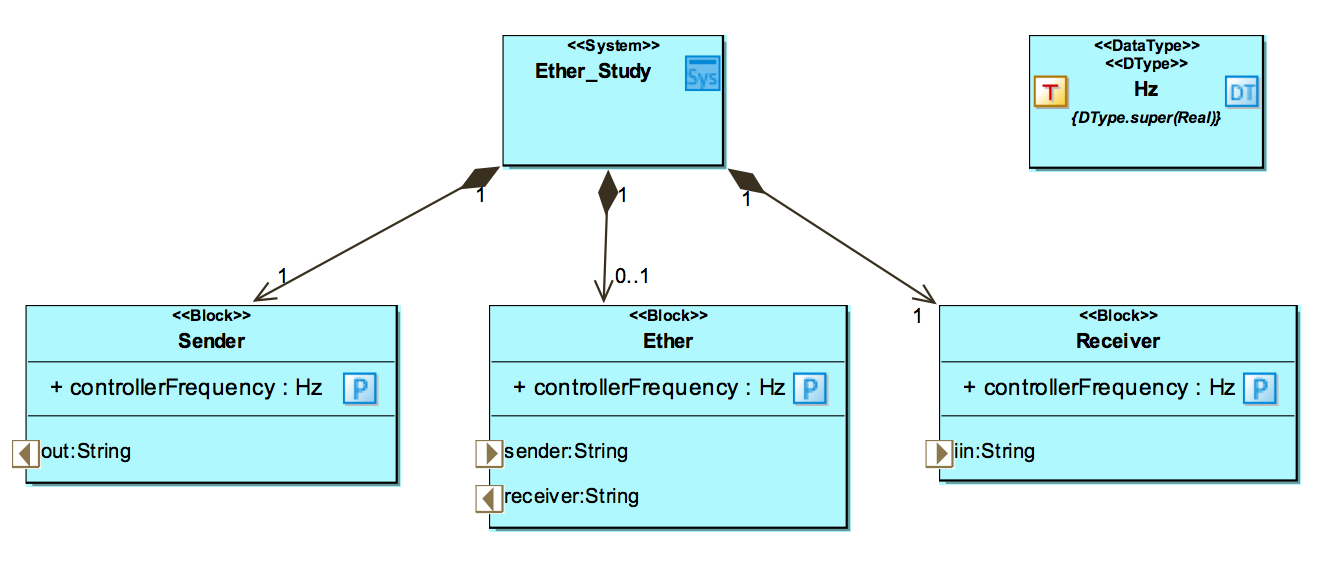
\includegraphics[scale=0.3]{figures/ether_asd}
\caption{\emph{Case Study: Ether} example}
\label{fig:ether_asd}
\end{figure}

By encoding VDM values as strings, it is possible to define a simple broadcast ether that receives message strings on its input channel(s) and sends them to its output channel(s). As a concrete example, we consider the \emph{Case Study: Ether} (see Deliverable D3.5~\cite{INTOCPSD3.5}), which contains a \texttt{Sender}, a \texttt{Receiver} and an \texttt{Ether}, as depicted in Figure~\ref{fig:ether_asd}. In this example, the three FMUs have the following roles:

\begin{description}[noitemsep]
  \item[Sender] Generates random 3-tuple messages of type \texttt{real * real * real}, encodes them as strings using the \texttt{VDMUtil} library and puts them on its output port.
  \item[Receiver] Receives strings on its input port and tries to convert them to single messages of type \texttt{real * real * real} or to a sequence of messages of type of type \texttt{seq of (real * real * real)}.
  \item[Ether] Has an input port and output port, each assigned a unique identifier, i.e. as a \texttt{map Id to StringPort}. It also has a mapping of input to output ports as a set of pairs: \texttt{set of (Id * Id)}. It has a list that holds messages for each output destination, because multiple messages might arrive for one destination. It gathers messages from each input and passes them to the outputs defined in the above mapping.
\end{description}

In this simple example, the sender and receiver are asymmetrical, but in more complicated examples controllers can be both senders and receivers by implementing both of the behaviours described above.

The \emph{Case Study: Ether} example contains two multi-models that allow the sender and receiver to be connected directly (connection diagram shown in Figure~\ref{fig:snd_rec}), or to be connected via the ether (connection diagram shown in Figure~\ref{fig:snd_ether_rec}). The description in the Examples Compendium, Deliverable D3.5~\cite{INTOCPSD3.5}, explains how to run the two different multi-models. This approach shows that the use of string ports and the \texttt{VDMUtil} library can be useful even without the ether for message passing between controllers in simple topologies.

For the sender, this connection is transparent, it does not care whether it is connected to the ether or not. For the receiver, in the direct connection it will receive single messages, whereas when receiving from the ether it will receive a list of messages (even for a single value). So the receiver is able to deduce when it is directly connected or connected via the ether. %Later in this section, when we describe quality of service, it is n



\begin{figure}
\begin{center}
\subfigure[Connection diagram of the \emph{Direct} multi-model in the \emph{Case Study: Ether} example]
{
	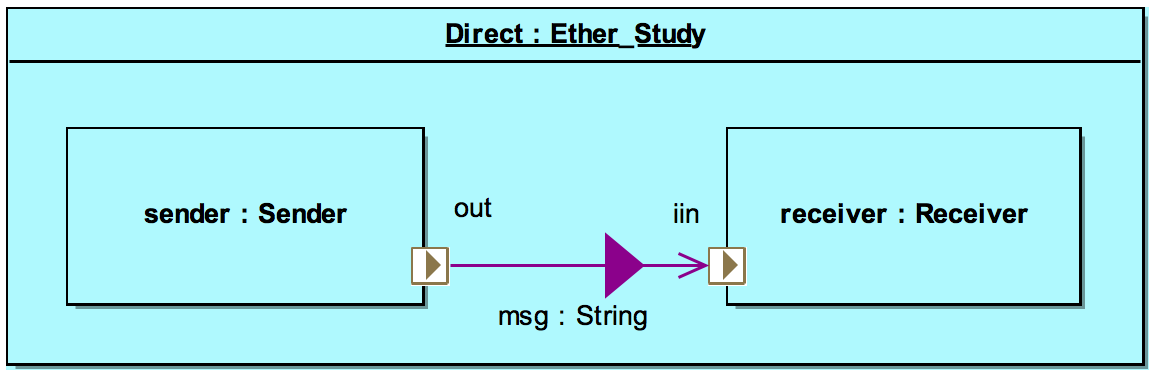
\includegraphics[scale=0.2]{figures/ether_cd_direct}
	\label{fig:snd_rec}
}
\subfigure[Connection diagram of the \emph{Ether} multi-model in the \emph{Case Study: Ether} example]
{
	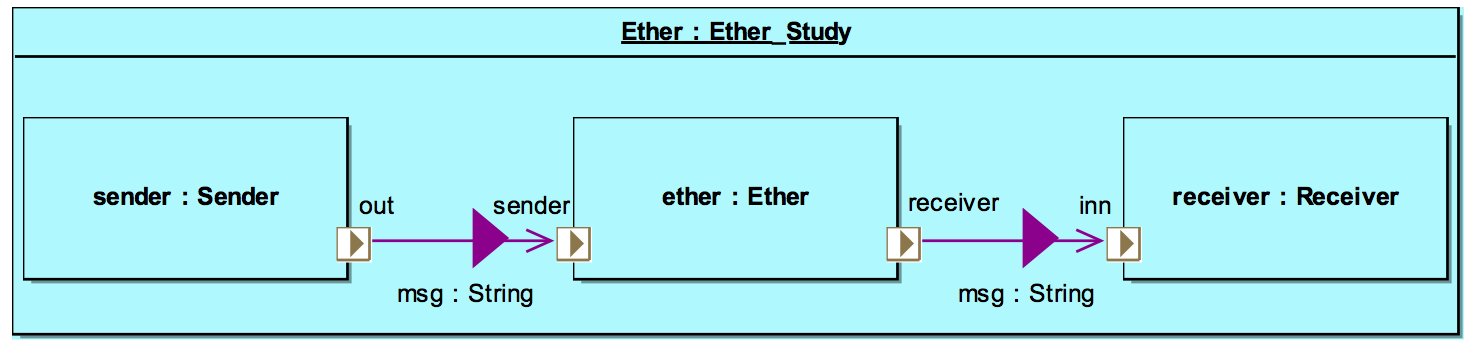
\includegraphics[scale=0.25]{figures/ether_cd_ether}
	\label{fig:snd_ether_rec}
}
\caption{Alternative multi-models in the \emph{Case Study: Ether} example}
\label{fig:cds}
\end{center}
\end{figure}

The ether defined in this example is intended to be generic enough that it can be used in other case studies that need a simple broadcast ether without guarantees of delivery. To use it, you can:

\begin{enumerate}[noitemsep]
\item Import the \emph{Ether} model from the \emph{case-study\_ether/Models} directory into Overture;
\item Update the \texttt{HardwareInterface}\footnote{A class that provides annotated definitions of the ports for a VDM FMU.} class to provide input and/or output ports for all controllers that will be connected to the ether.
\item Update the \texttt{System} class to assign identifiers to all input and output ports; and
\item Update the set of identifier pairs that define connections.
\end{enumerate}

\section{Consequences of Using the Ether}

The ether as presented above %, and listed in Appendix~\ref{app:ether},
is fairly basic. In each update cycle, it passes values from its input variables to their respective output variables. This essentially replicates the shared variable style of direct FMU-FMU connections, which means that the relative update speeds of the FMUs may lead to the following:

\begin{description}[noitemsep]
  \item[Values may be delayed] The introduction of an intermediate FMU means that an extra update cycle is required to pass values from sender to ether and ether to receiver. This may delay messages unless the ether updates at least twice as fast as the receiver.
  \item[Values may not be read] If a value is not read by the receiver before it is changed, then that value is lost.
  \item[Values may be read more than once] If a value is not changed by the sender before the receiver updates, then the value is read twice. In the simple ether, the receiver cannot distinguish an old message from a new message with the same values.
\end{description}

In the Examples Compendium, Deliverable D3.5~\cite{INTOCPSD3.5}, the \emph{Case Study: Ether} example is described along with some suggested experiments to see the effects of the above examples by changing the controller frequency parameters of the sender, ether and receiver. In the final part of this section we outline ways to overcome such problems if it is necessary to guarantee that messages arrive and are read during a co-simulation.

\section{Modelling True Message Passing and Quality of Service}

The key to achieving a true message-passing is to overcome the problem of distinguishing old messages from new messages with the same values. This can be done by attaching a unique identifier to each message, which could be, for example, an identifier of the sender plus a message number:

\newpage
\begin{vdm}
instance variables

id: seq of char := "a";
seqn: nat1 := 1;

...

VDMUtil`val2seq_of_char[seq of char*real*real](
  mk_(id ^ [seqn], 2.4, 1.5));
seqn := seqn + 1
\end{vdm}

The advantage of assigning an identifier to each controller is that messages could also contain destination addresses, instead of the broadcast model presented above. In order to achieve these, some changes are needed to allow for acknowledging receipt of messages. Controllers should:

\begin{enumerate}[noitemsep]
\item Send a queue of messages on their output channel along with message identifiers of (recently received) messages;
\item Expect to receive a queue of messages along with message identifiers of successfully sent messages; and
\item Senders should remove messages from their output queue once their receipt has been acknowledged.
\end{enumerate}

The \texttt{Ether} class must be extended to:

\begin{enumerate}[noitemsep]
\item Inspect the message identifier (and destination if required) using \texttt{VDMUtil};
\item Pass message identifiers back to senders to acknowledge receipts; and
\item Listen for message identifiers from receivers to know when to remove messages from the queue.
\end{enumerate}

A dedicated channel for acknowledging messages could also be introduced, which would simplify the above. Therefore, each controller would have four connections to the ether: send and acknowledge, receive and acknowledge, as depicted in Figure~\ref{fig:ack}.

\begin{figure}
\centering
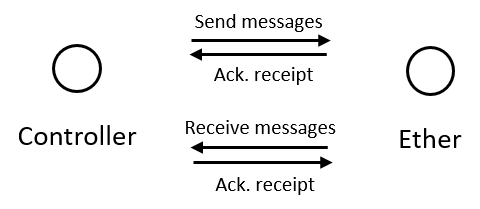
\includegraphics[scale=0.6]{figures/ack_channel}
\caption{Topology of controller to \emph{Ether} connection with dedicated channels for messages and acknowledgements}
\label{fig:ack}
\end{figure}

The advantages of guaranteed message delivery as described here are that realistic and faulty behaviour of the communication medium can be studied. An ether can be produced that provides poorer quality of service (delay, loss, repetition, reordering). These behaviours could be parameterised and explored using DSE (see Chapter~\ref{sec:dse}). By controlling for problems introduced by the nature of co-simulation, any reduction in performance of the multi-model can be attributed to the realistic behaviour introduced intentionally into the model of communications.

